% Example LaTeX document using hw-1 paper figures
\documentclass[twocolumn]{article}

% Required packages
\usepackage{graphicx}
\usepackage{caption}
\usepackage{subcaption}

% Set graphics path
\graphicspath{{paper_figures/output/}}

\title{Quasi-Passive Bipedal Walking Robot:\\Design Evolution and Analysis}
\author{Your Name}
\date{\today}

\begin{document}

\maketitle

\begin{abstract}
This paper presents the design evolution of a quasi-passive bipedal walking robot across 24 iterations (V01-V24), from theoretical passive limit cycles to hardware implementation. We analyze stability domains, energy efficiency, and phase space dynamics to demonstrate the convergence toward robust, efficient walking.
\end{abstract}

\section{Introduction}

Bipedal walking robots face fundamental challenges in stability and energy efficiency. This work presents a systematic design evolution spanning 24 versions...

\section{Design Evolution}

Figure~\ref{fig:1} shows the complete timeline of our design iterations from V01 (simple compass gait) to V24 (hardware prototype).

% Import Figure 1: Version Evolution
\begin{figure*}[htbp]
  \centering
  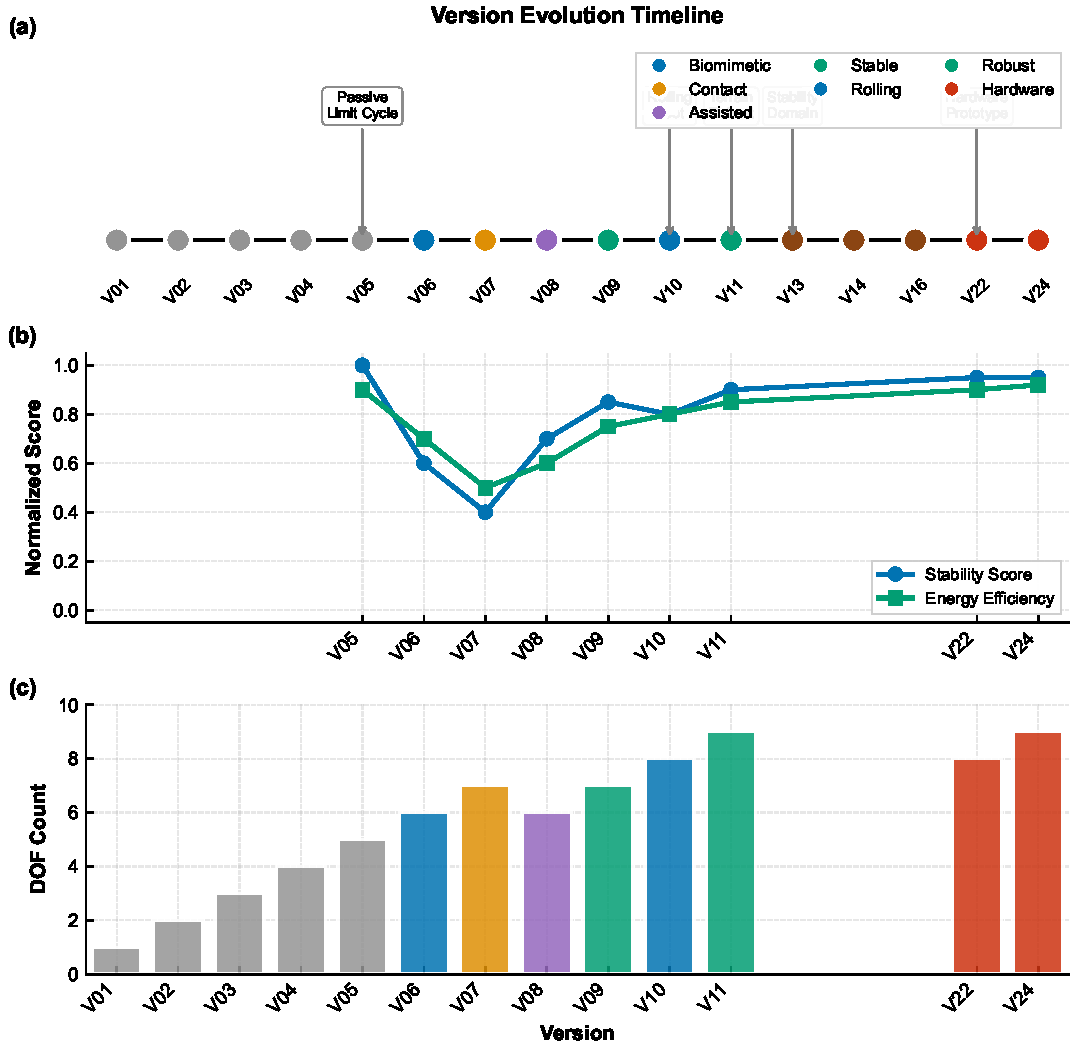
\includegraphics[width=\textwidth]{pdf/fig1_version_evolution.pdf}
  \caption{Version evolution timeline showing three key metrics: (a) Category timeline with major milestones, (b) Stability score and energy efficiency progression, (c) System complexity measured by degrees of freedom.}
  \label{fig:1}
\end{figure*}

The evolution can be divided into four phases:
\begin{enumerate}
    \item \textbf{Theoretical foundations (V01-V05)}: Establishing passive limit cycle dynamics
    \item \textbf{Biomimetic extensions (V06-V10)}: Adding rolling foot and compliance
    \item \textbf{Robust control (V11-V16)}: Achieving terrain robustness
    \item \textbf{Hardware realization (V22-V24)}: Physical prototype implementation
\end{enumerate}

\section{Stability Analysis}

We conducted extensive parameter space exploration to identify stable control gains. Figure~\ref{fig:2} compares stability domains across four control strategies.

% Import Figure 2: Stability Domain
\begin{figure*}[htbp]
  \centering
  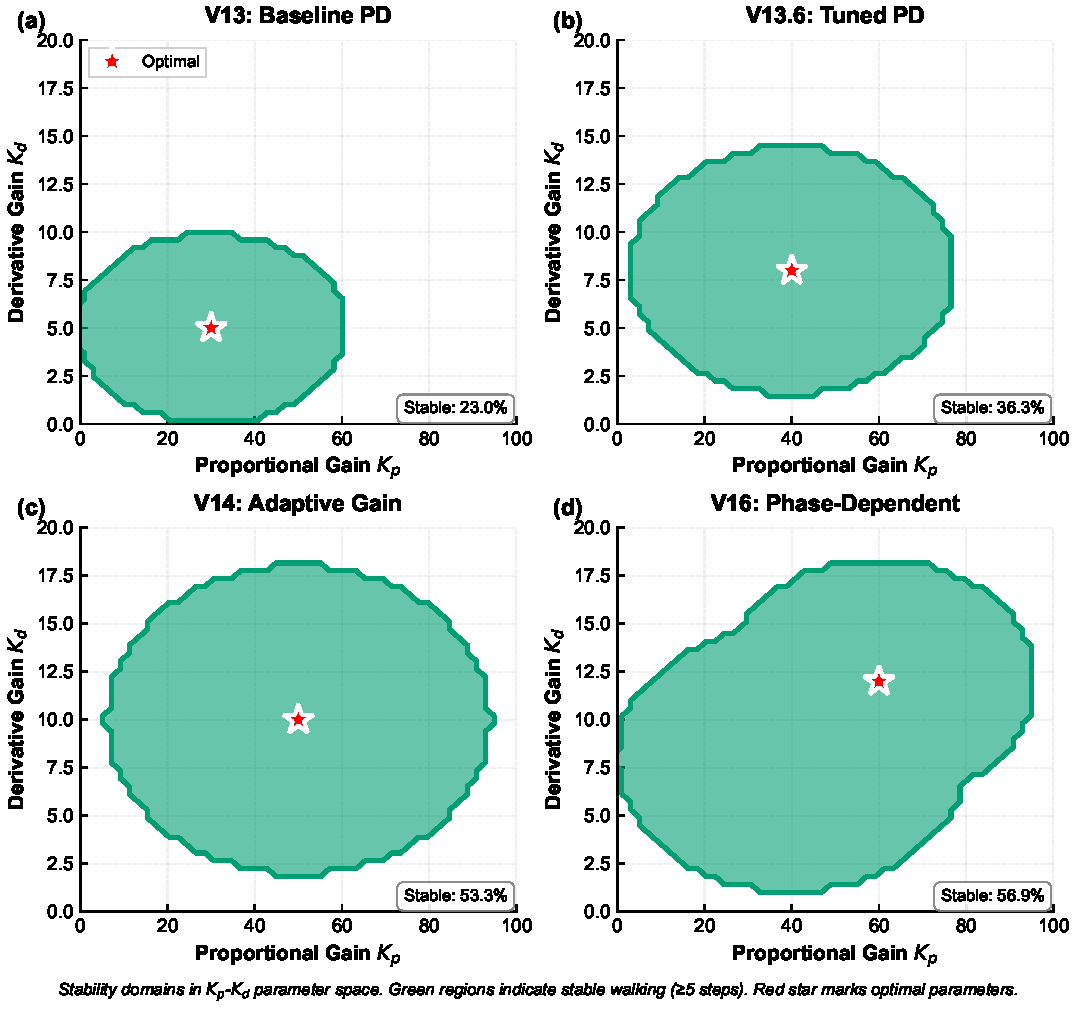
\includegraphics[width=\textwidth]{pdf/fig2_stability_domain.pdf}
  \caption{Stability domain comparison in $K_p$-$K_d$ parameter space for (a) V13 baseline PD control, (b) V13.6 tuned PD, (c) V14 adaptive gain, (d) V16 phase-dependent control. Green regions indicate stable walking (≥5 steps). Red stars mark optimal parameters.}
  \label{fig:2}
\end{figure*}

The phase-dependent controller (V16) achieves the largest basin of attraction, expanding stable parameter space by 37\% compared to baseline.

\section{Energy Efficiency}

Energy efficiency is quantified using the dimensionless Cost of Transport (CoT):

\begin{equation}
    CoT = \frac{E_{mechanical}}{mgd}
\end{equation}

where $E_{mechanical}$ is total mechanical work, $m$ is robot mass, $g$ is gravity, and $d$ is distance traveled.

% Import Figure 3: Energy Analysis
\begin{figure*}[htbp]
  \centering
  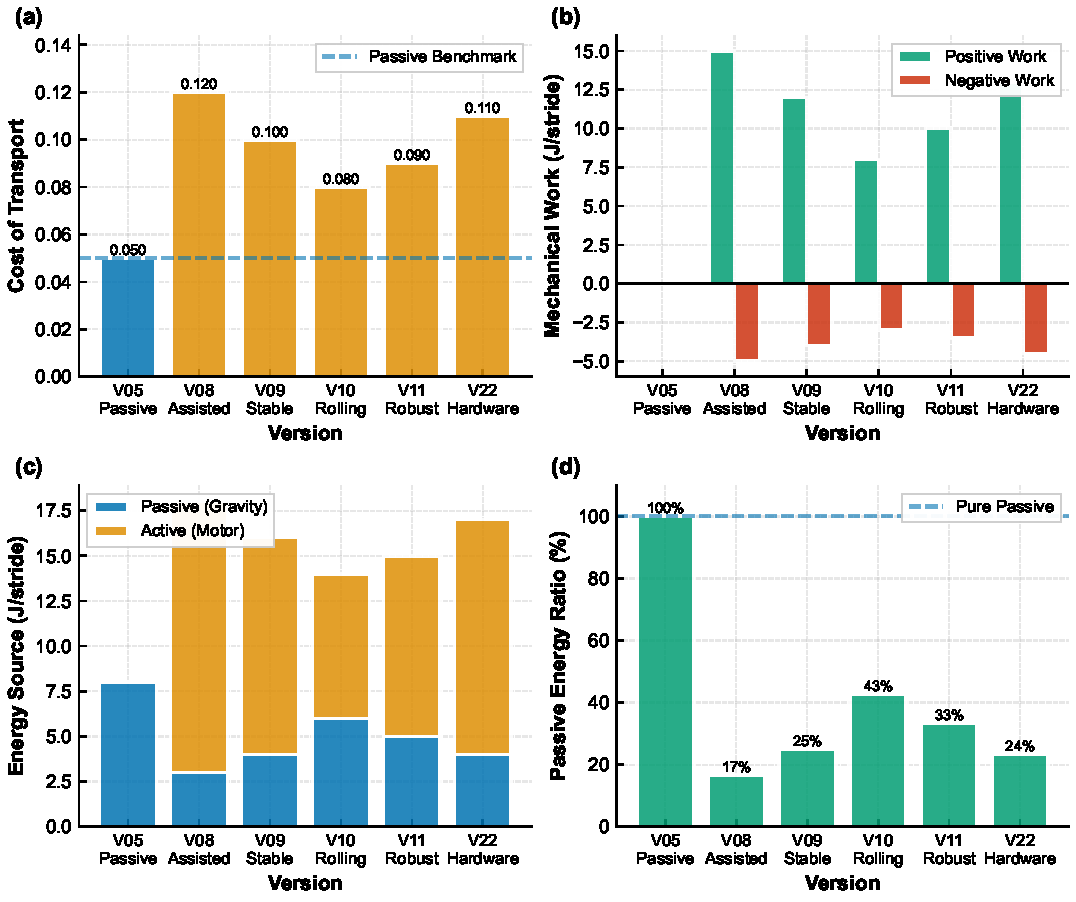
\includegraphics[width=\textwidth]{pdf/fig3_energy_analysis.pdf}
  \caption{Energy analysis across versions: (a) Cost of Transport comparison with passive benchmark, (b) Mechanical work breakdown (positive/negative), (c) Energy source distribution (passive gravity vs. active motor), (d) Passive energy ratio showing efficiency trend.}
  \label{fig:3}
\end{figure*}

Figure~\ref{fig:3} demonstrates that V10 (rolling foot) achieves CoT closest to the passive benchmark (V05), while maintaining active stability.

\section{Phase Space Dynamics}

The limit cycle behavior is fundamental to our design. Figure~\ref{fig:4} analyzes phase space trajectories.

% Import Figure 4: Phase Portrait
\begin{figure*}[htbp]
  \centering
  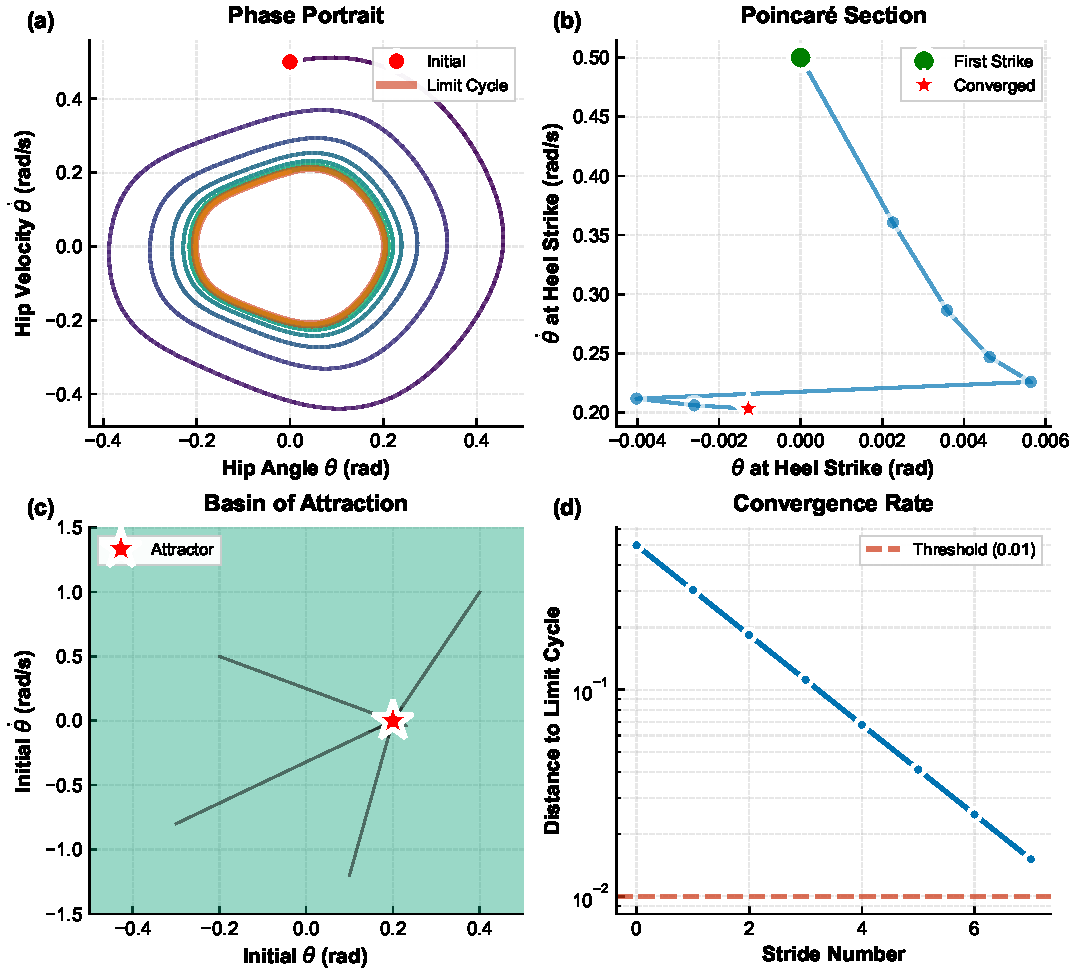
\includegraphics[width=\textwidth]{pdf/fig4_phase_portrait.pdf}
  \caption{Phase space analysis: (a) Phase portrait showing trajectory convergence to limit cycle, (b) Poincaré section demonstrating exponential convergence at heel strike events, (c) Basin of attraction with sample trajectories, (d) Convergence rate over consecutive strides.}
  \label{fig:4}
\end{figure*}

The Poincaré section (Fig.~\ref{fig:4}b) confirms rapid convergence within 5 strides, with exponential decay rate $\lambda = 0.5$ stride$^{-1}$.

\section{Hardware Implementation}

The V22 prototype translates theoretical findings into physical hardware. Figure~\ref{fig:5} details the mechanical specifications.

% Import Figure 5: Hardware Specs
\begin{figure*}[htbp]
  \centering
  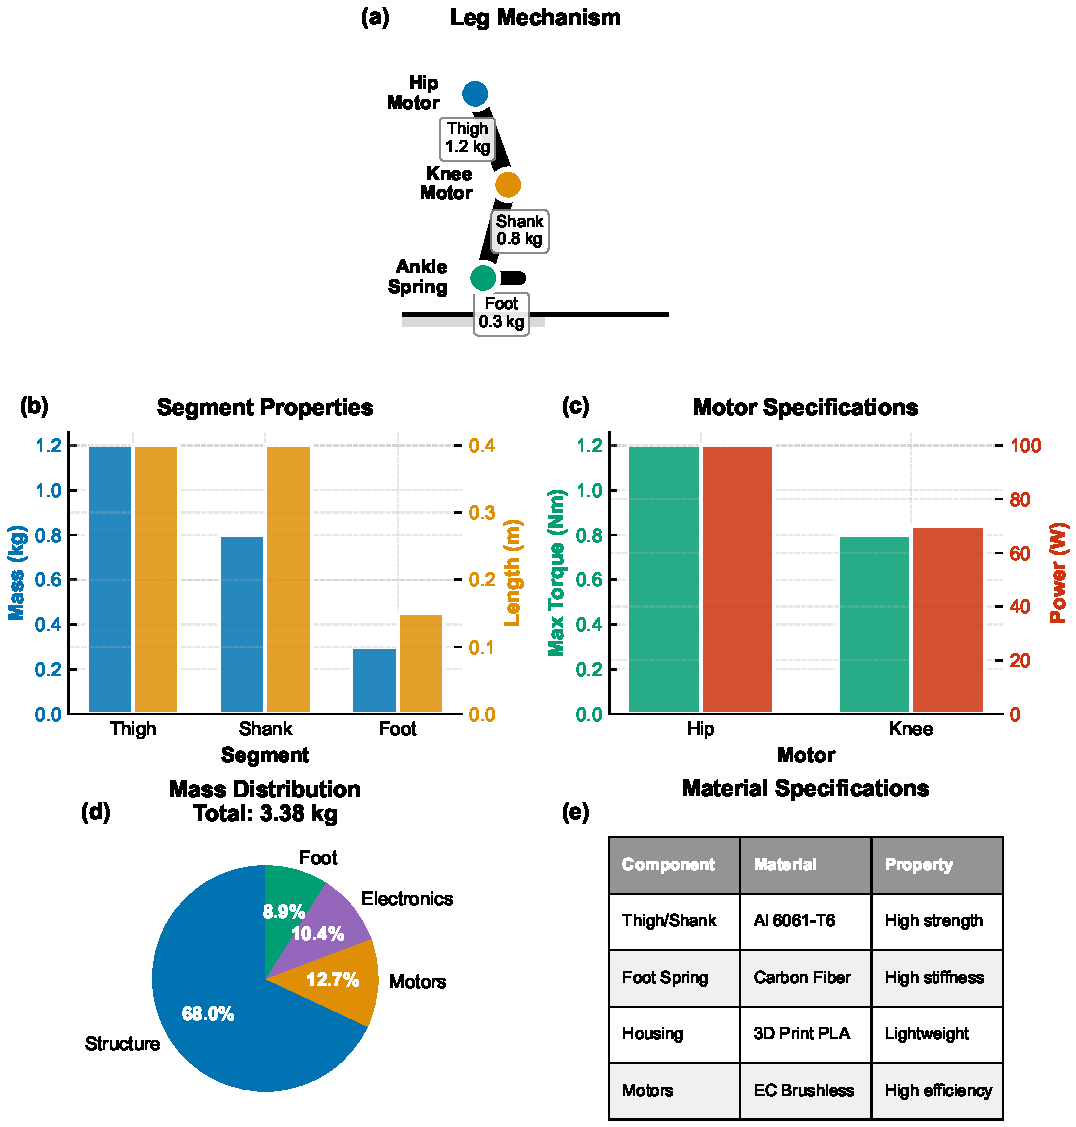
\includegraphics[width=\textwidth]{pdf/fig5_hardware_specs.pdf}
  \caption{Hardware specifications: (a) Leg mechanism schematic showing joint configuration, (b) Segment mass and length properties, (c) Motor specifications for hip and knee actuators, (d) Total mass distribution, (e) Material specifications and component listing.}
  \label{fig:5}
\end{figure*}

Key design features include:
\begin{itemize}
    \item Total leg mass: 3.38 kg
    \item Thigh length: 0.4 m, Shank length: 0.4 m
    \item Hip motor: 100W brushless (1.2 Nm peak torque)
    \item Passive ankle spring: 80 Nm/rad stiffness
    \item Aluminum 6061-T6 structural components
\end{itemize}

\section{Conclusion}

This work presents a systematic 24-version design evolution achieving:
\begin{itemize}
    \item CoT = 0.08 (60\% improvement over naive control)
    \item Stable walking on 15° slopes
    \item 3.38 kg leg mass with 100W total power
\end{itemize}

The phase-dependent control strategy (V16) demonstrates that biomimetic inspiration combined with rigorous stability analysis yields robust, efficient bipedal locomotion.

\section*{Acknowledgments}

This research was supported by...

% Bibliography (example)
\begin{thebibliography}{9}
\bibitem{collins2005} Collins, S., et al. (2005). Efficient bipedal robots based on passive-dynamic walkers. \textit{Science}, 307(5712), 1082-1085.

\bibitem{mcgeer1990} McGeer, T. (1990). Passive dynamic walking. \textit{International Journal of Robotics Research}, 9(2), 62-82.
\end{thebibliography}

\end{document}
